% \begin{figure}[htbp]
% \centering
% 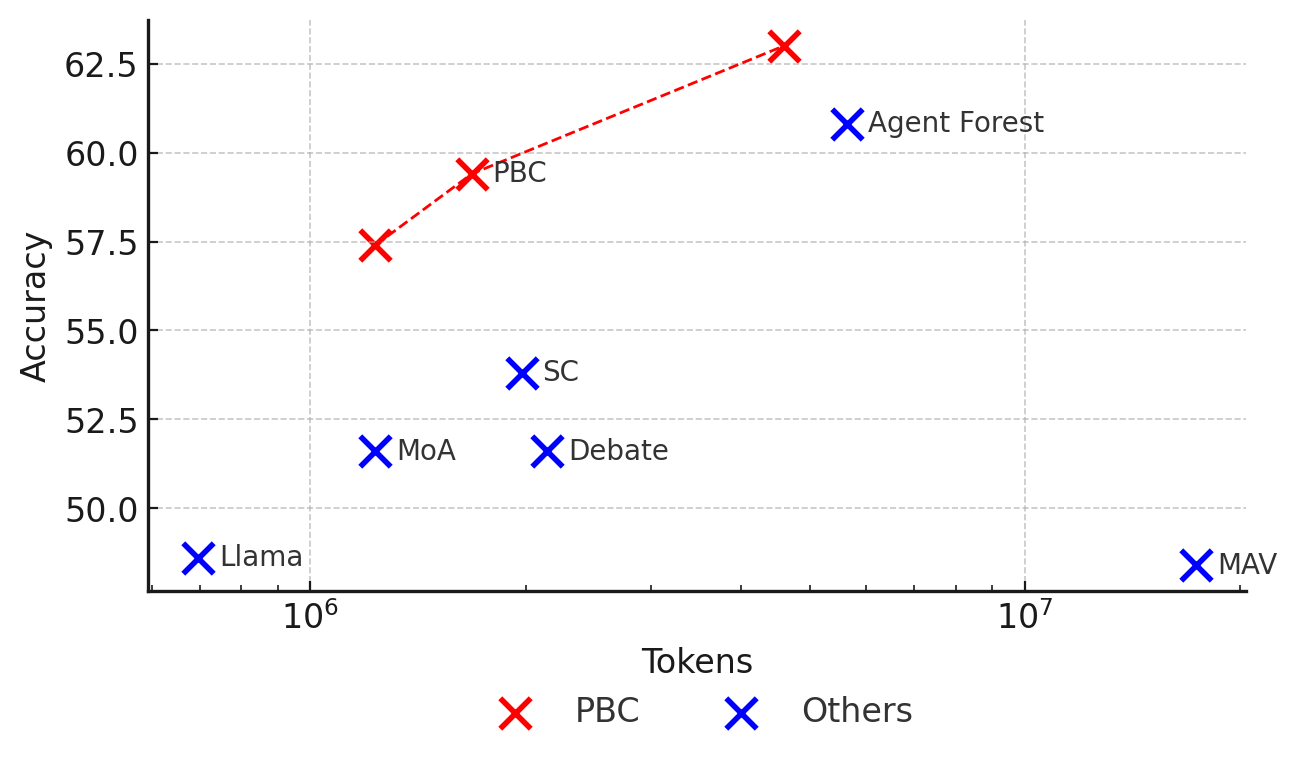
\includegraphics[width=0.8\linewidth]{Figures/Scatter_v1.png}
% \caption{\textbf{Token usage versus accuracy.} on the \textsc{MATH} dataset. Red markers denote the performance of our Protocol-based composition (\NAME{}) method built from three small models.}
% \label{fig:token-accuracy}
% \end{figure}

% For years, the path to more capable Large Language Models (LLMs) has been to relentlessly increase model parameters and data volume, resulting in models with trillions of parameters. Yet, the long-term sustainability of this scaling-first strategy is now in question. It faces two critical constraints: the prohibitive cost of computation and the finite supply of high-quality text data. With these bottlenecks, the returns from scaling are diminishing.

% At the same time, there has also been a surge of small-sized models in the range of a few billion to a few dozen billion parameters. These models are not state-of-the-art in terms of performance, but they offer much lower inference costs compared with the largest frontier systems. Moreover, different models also bring different capabilities.

Recent years have witnessed a surge of small-sized language models (SLMs) containing billions to tens of billions of parameters~\citep{wang2024comprehensivesurveysmalllanguage, javaheripi2023phi, guo2025deepseek, allal2025smollm2}. While these models may underperform state-of-the-art frontier language models, which usually contain hundreds of billions to trillions of parameters, on any given query, they offer substantially lower inference costs, are more affordable to train and finetune, and allow edge deployment due to their small size~\citep{belcak2025small}.  
Meanwhile, frontier models have reached trillion-parameter scales where further increases in size and training data yield diminishing returns. This mirrors a well-known challenge in computer architecture two decades ago: when enlarging single CPU cores no longer delivered proportional performance gains, computer architects turned to designing multi-core processors, where multiple smaller cores working together enabled sustained improvements.  This parallel suggests that combining multiple SLMs could offer a promising alternative to scaling ever-larger frontier models.


% This mirrors a well-known challenge in computer architecture two decades ago: when enlarging single CPU cores no longer delivered proportional performance gains, computer architects turned to designing multi-core processors, where multiple smaller cores working together enabled sustained improvements. 

% This parallel suggests that combining multiple SLMs could offer a promising alternative to scaling ever-larger frontier models. %This raises the question: would the field benefit more from an analogous architectural transition, shifting focus from developing increasingly large frontier models to optimizing ensembles of heterogeneous SLMs?%

% \cw{add GPT 5 into intro, add overall story on top}
% While scaling up model parameters and training data volume has historically been the primary route to stronger language models (LLMs), this strategy is increasingly constrained by hardware bottlenecks—such as limited GPU supply, a looming shortage of high-quality human-generated text, and diminishing performance gains at extreme scale. As a result, alternative approaches beyond brute-force scaling are becoming crucial for future progress.~\citep{scalinglaw,villalobos2024rundatalimitsllm,nellis2024nvidia}.

% At the same time, there has also been a surge of small-sized models in the range of a few billion to a few dozen billion parameters. These models are not state-of-the-art in terms of performance, but they offer much lower inference costs compared with the largest frontier systems. Moreover, different models also bring different capabilities, with their own strengths that make them valuable in specific contexts.

% Given these trends, a promising direction of research involves composing existing language models to create a more powerful ensemble. The central idea behind such compositional approaches is that different LLMs excel in different areas. By constructing a multi-model system that strategically integrates these individual strengths, the combined system can achieve performance levels exceeding those of any single model used alone, especially in more complex tasks~\citep{smit2024goingmadlookmultiagent,li2024agentsneed}. This method presents an opportunity to advance model capabilities without the significant costs and resources associated with continually scaling up a single model.

% Recently, several works have explored the composition of different language models. However, these approaches have predominantly focused on ensembles of state-of-the-art LLMs, which typically consist of models with tens to hundreds of billions of parameters. The composition in these frameworks is often realized through communication between the models. Given that these large models already possess strong individual capabilities and a high degree of instruction-following proficiency, they can collaborate effectively. In contrast, these works generally do not discuss the application of such compositional methods to smaller models—those in the few to tens of billions of parameters range. Furthermore, our preliminary investigations suggest that directly porting these existing techniques to smaller-scale models often fails to produce the desired performance gains.


%One line of work relies on router-based systems, where an auxiliary model or heuristic directs each query to the most appropriate LLM (\cite{openai_gpt5_2025, ong2024routellm, yue2025masrouter})). While effective, these methods typically require training or maintaining specialized routing models, which constrains their applicability in many scenarios and makes them less relevant for our setting.

Recent works have explored orchestrating multiple LLMs (e.g., GPT-3.5 and GPT-4o), combining them into one system to process an input collaboratively. Representative approaches include Mixture-of-Agent~\citep{wang2024mixtureofagentsenhanceslargelanguage}, LLM-Debate~\citep{du2023improvingfactualityreasoninglanguage}, and Multi-Agent Verification~\citep{lifshitz2025multiagentverificationscalingtesttime}. These approaches share a key assumption: that models possess strong reasoning and deliberation abilities, so that interaction through natural language can reliably correct mistakes. However, when applied to SLMs, this assumption no longer holds. Our study finds that \emph{such discussion-based orchestration often fails to improve performance for SLMs}, and in some cases even reduces accuracy by over 5\%. Instead of correcting mistakes, SLMs tend to fall into groupthink during interaction, amplifying errors rather than mitigating them. The assumptions that language models can correct each other's answers behind existing orchestration methods do not hold for SLMs~\citep{Taubenfeld_2024,huang2024largelanguagemodelsselfcorrect,liu2023lostmiddlelanguagemodels}. 


% Several recent works have explored combining different LLMs (such as GPT-3.5 and GPT-4) to improve model performance 
%  via structured discussion frameworks, where multiple LLMs interact to verify and refine each other’s answers (\cite{wang2024mixtureofagentsenhanceslargelanguage, pitre2025consensagent, du2023improvingfactualityreasoninglanguage}). For example, LLM-debate \citep{du2023improvingfactualityreasoninglanguage} proposes that model instances first produce individual responses and then engage in deliberation to converge on a common answer. These approaches heavily on models’ ability to engage in effective deliberation -- a capability that, as we analyze, remains limited in small-sized models. 

%For instance, OpenAI's latest model as of August 2025, GPT-5, consists of multiple language models; \citep{du2023improvingfactualityreasoninglanguage} proposed LLM-debate, an approach to improve language responses by having multiple language model instances individually propose and jointly debate their responses to arrive at a common answer.%


%Besides, SLMs often show complementary strengths, with each excelling on particular types of queries~\citep{ong2025routellmlearningroutellms}. Such heterogeneity may provide an advantage of combining multiple SLMs for inference. 


%Our analysis indicates that the ineffectiveness of these existing discussion-based methods in small size models stems from the weak cognitive abilities of SLMs. SLMs are weak in abilities such as reflection, verification, and distinguishing right from wrong when given a mixed answer. As a result, they cannot effectively learn from other language models. Our experimental results show that a debate between such small models usually leads to amplifying the wrong answer rather than finding the right one. Additionally, existing works on discussion-based methods often focus on proposing an architecture and demonstrating a prototype. However, they rarely address how such architectures can be easily adapted or improved across different domains.

% On the other hand, small-sized language models are also weak in their long-context ability. They struggle to effectively process the dynamic discussion among models.For some small-sized models, the context easily exceeds max allowed when using them to discuss with each other. Consequently, they have to rely on a fixed, pre-written prompt, which hinders them from eliciting their heterogeneous abilities.

% In this work, we propose \textbf{\NAME{}}, a multi-model architecture for effectively orchestrating SLMs while avoiding explicit text exchanges between models. Our key insight is that while prior discussion-based methods assume models possess complementary abilities and can learn through text communication, small-sized models actually fail in this paradigm, where text communication amplifies rather than corrects errors. \NAME{} leverages model heterogeneity by selecting outputs based on confidence scores without any model training. 

To address this issue, we propose \textbf{\NAME{}}, a multi-model architecture for effectively orchestrating SLMs while avoiding explicit text exchanges between models. Our key insight is that \NAME{} leverages complementary abilities from different models by selecting outputs based on confidence scores without any model training.


% To address this challenge, we introduce \textbf{\NAME{}}, a multi-model architecture that effectively coordinates multiple SLM for enhanced reasoning. Unlike prior approaches that rely on explicit discussions between models, \NAME{} estimates each model’s confidence using simple rules, without requiring inter-model text exchange. The system then selects the final output based on the confidence of models.


\begin{wrapfigure}{r}{0.5\linewidth}
  \centering
  \vspace{-5pt}
  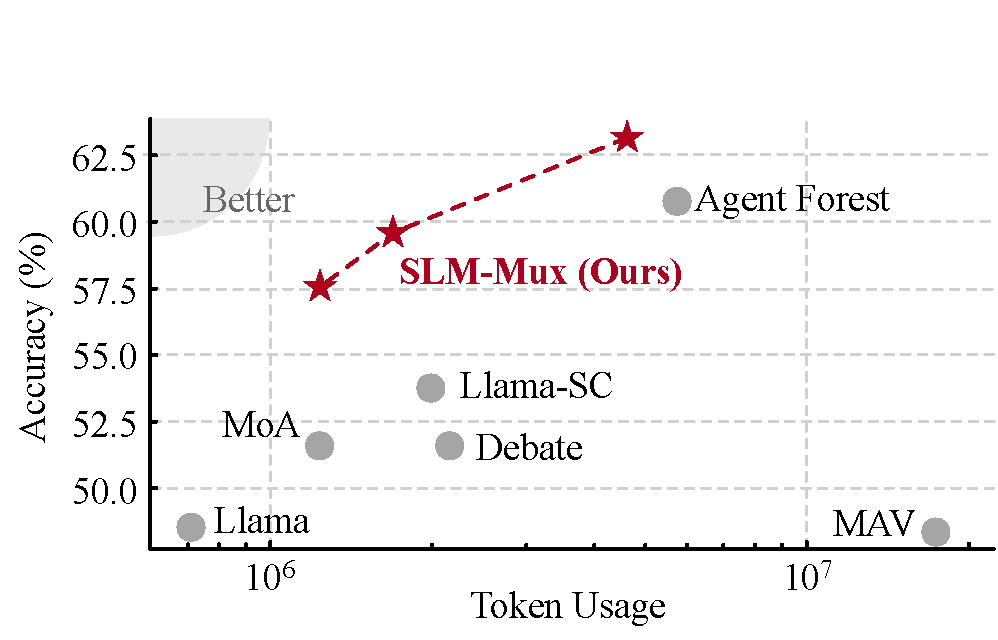
\includegraphics[width=\linewidth]{Figures/scatter_v3.pdf}
  \vspace{-15pt}
  \caption{\small \textbf{Head-to-Head Comparison of \NAME{} with Other Methods.} \NAME{} outperforms existing methods such as Self-Consistency (SC)~\citep{wang2023selfconsistencyimproveschainthought}, Mixture-of-Agents (MoA)~\citep{wang2024mixtureofagentsenhanceslargelanguage}, LLM-Debate~\citep{du2023improvingfactualityreasoninglanguage}, Multi-Agent Verification (MAV)~\citep{lifshitz2025multiagentverificationscalingtesttime}, and Agent Forest~\citep{li2024agentsneed}. Results reported on \textsc{MATH} dataset with SLMs.}
  \label{fig:token-accuracy}
  \vspace{-20pt}
\end{wrapfigure}

% After we have the \NAME{}, the next question emerges: with dozens of SLMs now available, we
% have access to a large model pool.  Since it is not feasible to invoke every SLM in the \NAME{}
% architecture for every given query, it is worth investigating whether there is an optimal strategy for
% selecting a limited subset of models for each task. On the other hand, model selection quality may impact the performance of \NAME{}.  For example, as shown in Figure~\ref{fig:motivation-search}, the two models on the left have no complementary capabilities. Llama 3.2 3B offers no advantage in every subject: for most (if not all) MATH questions, if Qwen 2.5 7B cannot solve them, neither can Llama 3.2 3B. In this case, combining them provides no benefit. However, the models on the right show complementary strengths: Mistral Small 24B scores higher in some subjects, and Qwen 2.5 7B does better in others. In this case, when Qwen 2.5 7B cannot answer a question, Mistral Small 24B may succeed.

After introducing \NAME{}, another question arises: which models should be orchestrated together? Not all combinations are effective -- if one model is weaker across all dimensions, it provides no benefit when paired with a stronger one. In contrast, combining models with complementary strengths (e.g., one stronger in algebra, another in geometry) allows the system to succeed where a single model would fail.

To address this, we develop a \textbf{model selection search strategy} for \NAME{}, which systematically evaluates and identifies model subsets with complementary strengths. By maximizing union accuracy while penalizing overconfident contradictions, the search procedure finds the most suitable models for a given model budget. 

In addition, we explore \textbf{compute scaling strategies} for the selected model ensembles to further enhance performance. By adjusting the number of models and samples at inference time, we further boost performance and identify practical sweet spots in the accuracy-compute tradeoff.


% We further develop an optimization strategy for model selection within the \NAME{} framework. Our method systematically identifies model combinations that maximize complementarity among small-sized LLMs, enabling us to achieve higher accuracy with minimal computational overhead by using only two or three models. This principled selection process ensures optimal performance while maintaining the efficiency advantages of SLMs.

% Second, to tackle the challenge of eliciting heterogeneous abilities with fixed prompts, we propose an inference-time prompt tuning method. This method specializes the prompt for each model to activate its unique strengths for a given query. By ensuring the models provide complementary abilities, the overall accuracy of the ensemble is significantly improved.

% second, we proposed a method to optimize \NAME{}. We  propose an method to select models based on their heterogeneity and maximize their heterogeneity between small-sized LLMs. 

Our experiments demonstrate significant improvements across multiple benchmarks. By combining only two SLMs, we achieve accuracy improvements of up to 6.7\% on MATH, 5.7\% on GPQA, and 4.8\% on GSM8K, compared to the best-performing single SLMs in the system. Our method consistently outperforms existing discussion-based approaches for SLMs, with gains of up to 13.4\% on MATH, 8.8\% on GPQA, and 7.0\% on GSM8K. Most importantly,  with just two SLMs, \NAME{}  outperforms Qwen 2.5 72B on GPQA and GSM, and matches its performance on MATH.

% \cw{Problem formulation: how to find a good performing SLM ensemble? }

Finally, we complement these empirical findings with theoretical and experimental analyses. Our approach shows superiority in multiple scenarios compared with previous methods (Figure \ref{fig:token-accuracy}). 

Our main contributions are as follows:
% :
% \begin{itemize}
% \begin{itemize}[leftmargin=2em, nosep]
% \item[{\bf i)}] We revisit the problem of multi-model composition with small-sized LLMs, and show that limited cognitive ability is a key factor underlying the failure of prior discussion-based methods.
% 
% \item[{\bf i)}] We propose Protocol-Based Composition (\NAME{}), a novel architecture that improves the compositional performance of small-sized models, achieving more accurate and efficient ensembles compared to prior approaches.
% 
% \item[{\bf i)}]
\textbf{ (i) We identify a fundamental limitation of existing orchestration methods:} Through systematic evaluation, we demonstrate that existing discussion-based methods, which show consistent improvements for frontier LLMs, actually harm performance when applied to SLMs. This counterintuitive finding challenges the assumption that orchestration methods transfer across model scales and reveals the need for SLM-specific method.
% 
% 
% \item[{\bf ii)}] We develop a model selection optimization technique that further improves the effectiveness of the proposed \NAME{} framework by enabling more principled and accurate selection of models.
% 
% 
% \item[{\bf ii)}] 
\textbf{(ii) We propose \NAME{}}, a novel multi-model architecture designed specifically for SLMs that avoids the error amplification problems of discussion-based methods. \NAME{}{} achieves consistent gains across multiple benchmarks (MATH, GPQA, GSM8K) and significantly outperforms existing discussion-based methods by large margins (up to 11.6\% on MATH).
% 
% 
% \item[{\bf iii)}] We demonstrate that our method significantly improves the performance of SLMs, achieving consistent gains across multiple benchmarks (MATH, GPQA, GSM8K) and outperforming both discussion-based multi-model composition architectures by a large margin.
% 
% \item[{\bf iii)}] 
\textbf{(iii) We develop principled optimization strategies} for the \NAME{}, including model selection search that identifies complementary model selections and compute scaling strategies, further boosting performance while maintaining efficiency.
% 
% 
% \cw{TODO architecture definition; change into architecture}

% \item We conduct extensive ablation studies and theoretical analyses to demonstrate the effectiveness of our proposed methods.
% \end{itemize}

% The remainder of this paper is structured as follows. Section~\ref{sect:related} reviews related work. Section~\ref{sect:failure} analyzes the limitations of existing discussion-based approaches. Section~\ref{sect:method} presents our proposed protocol-based composition framework and its optimizations. Section~\ref{sect:experiment} reports experimental results, while Section~\ref{sect:analysis} provides theoretical and ablation analyses. Finally, Section~\ref{sect:conclusion} concludes the paper and outlines future directions.

 
% \cw{new paper outline intro, related, method 1 limitation, method 2 composition, method 3 optimization, experiment, analyze 1 theory, analyze 2 ablation study}

 

% One promising alternative to address these constraints is compositional language models, which leverage existing LLMs more effectively by orchestrating them in structured workflows. The central idea behind compositional language models is that different LLMs excel in different areas. By constructing a multi-model system that strategically integrates these individual strengths, the combined system can achieve performance levels exceeding those of any single model used alone, especially in more complex tasks~\citep{smit2024goingmadlookmultiagent,li2024agentsneed}.

% For instance, multiple models can iteratively debate and critique each other's proposed solutions to resolve disagreements and enhance accuracy~\citep{du2023improvingfactualityreasoninglanguage}; responses from diverse LLMs can be integrated to generate higher-quality, more useful answers~\citep{wang2024mixtureofagentsenhanceslargelanguage}; or several models may independently evaluate candidate answers and collectively select the best response, thus improving mathematical accuracy~\citep{lifshitz2025multiagentverificationscalingtesttime}. 

% However, existing composition methods generally rely on repeated calling advanced, state-of-the-art language models, each requiring costly API calls. Given that these models are already resource-intensive individually, orchestrating several of them improves the overall expense significantly compared to employing just a single model directly to generate an answer~\citep{wang2024rethinkingboundsllmreasoning,gandhi2025budgetmlagentcosteffectivellmmultiagent}. As a result, these methods are often expensive. Exisiting works don't explore composition of small models.

% However, existing compositional methods typically involve repeated API calls to advanced, state-of-the-art LLMs, each call incurring significant computational cost. Because each of these models individually already consumes substantial resources, combining multiple models can greatly amplify the overall cost compared to simply using a single model~\citep{wang2024rethinkingboundsllmreasoning,gandhi2025budgetmlagentcosteffectivellmmultiagent}. As a result, current methods become prohibitively expensive. Furthermore, prior research has generally overlooked exploring compositional approaches using smaller-scale, less costly models.

% \begin{wrapfigure}{r}{0.5\linewidth}
%   \centering
%   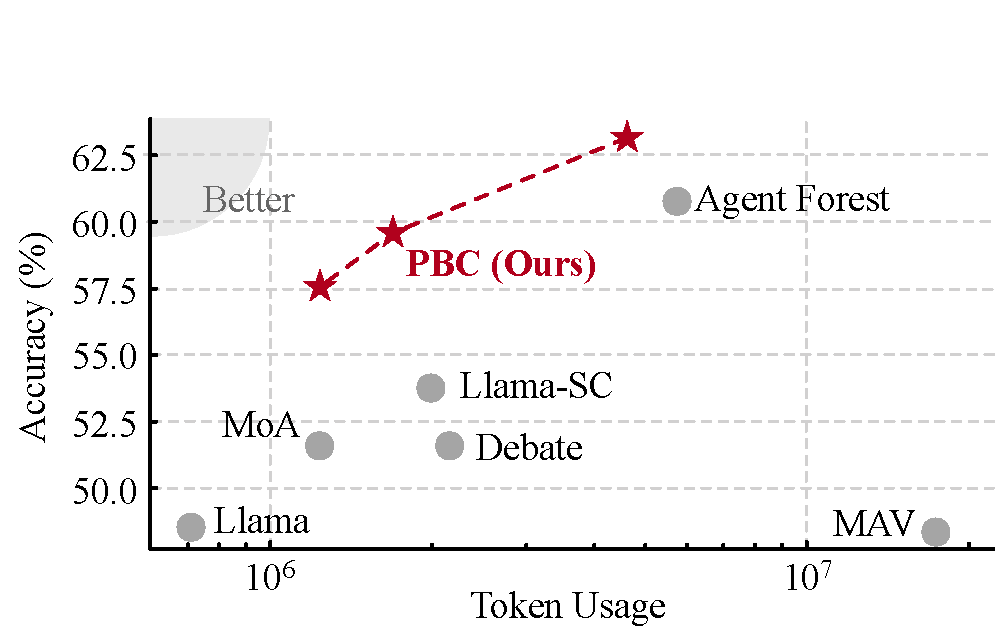
\includegraphics[width=\linewidth]{Figures/scatter_v2.pdf}
%   \vspace{-15pt}
%   \caption{\small \textbf{Protocol Based composition.} We present Protocol-based composition (\NAME{}), a new method to combine language models together which outperforms existing methods such as Self-Consistency (SC)~\citep{wang2023selfconsistencyimproveschainthought}, Mixture-of-Agents (MoA)~\citep{wang2024mixtureofagentsenhanceslargelanguage}, LLM-Debate~\citep{du2023improvingfactualityreasoninglanguage}, Multi-Agent Verification (MAV)~\citep{lifshitz2025multiagentverificationscalingtesttime}, and Agent Forest~\citep{li2024agentsneed}. Results reported on the \textsc{MATH} dataset with smaller-scale LLMs. }
%   \label{fig:token-accuracy}
%   \vspace{-10pt}
% \end{wrapfigure}

% Motivated by these observations, we explore whether it is possible to design a compositional method using smaller-scale, more economically friendly language models that can achieve similarly impressive performance improvements as those seen in larger-model systems, but at a lower cost. However, when directly applying existing compositional methods to smaller-scale models, we observed that the effectiveness of these methods is significantly reduced. This indicates that simply reusing current methods isn't sufficient—new approaches specifically designed for smaller-scale, economically friendly models are necessary.

% % Motivated by these cost and efficiency challenges, we investigate whether compositional language models constructed from smaller-scale, less resource-intensive models can achieve performance gains comparable to systems utilizing larger models. However, when directly applying smaller models within existing compositional methods, we observe a significant degradation in performance. Developing compositional methods specifically effective for smaller-scale models is not a straightforward task.

% % Although directly applying existing compositional methods to smaller language models usually leads to performance degradation, this issue is not insurmountable. Upon investigation, we attribute this decline primarily to two factors: superficial interactions between models and intrinsic capability limitations of smaller models themselves. Existing methods typically rely on sophisticated prompting techniques to facilitate interactions and aggregation of responses. However, these prompt-based interactions prove unstable and problematic for smaller models, hindering enhancement through interaction between models. Nonetheless, smaller models hold substantial compositional potential; we show that, theoretically, even three weak models (with accuracy <56\% on MATH~\citep{hendrycks2021measuringmathematicalproblemsolving} dataset) could significantly improve combined accuracy (64\%) if collected responses were perfectly selected. Motivated by this observation, we explore alternative compositional methods specifically tailored for smaller-scale models, proposing Protocol-based composition (\NAME{}) methods as a potentially more stable and effective alternative for smaller-scale models. Using our approach, we substantially improve the accuracy of smaller models, increasing their performance from below 56\% to approximately 63\%, closely approaching the theoretical upper limit.

% To understand why this performance gap arises, we analyzed the interactions among smaller-scale models. We found two main issues limiting their effectiveness: superficial interactions between models, and inherent capability constraints of smaller-scale models themselves. Existing compositional methods depend heavily on sophisticated prompting techniques, which are often problematic and ineffective for smaller-scale models. Despite these limitations, smaller-scale models still hold significant compositional potential. Our analysis shows that combining three relatively weak models—each with an average accuracy of around 46\% on the MATH dataset~\citep{hendrycks2021measuringmathematicalproblemsolving}—can theoretically achieve a combined accuracy of approximately 64\%, assuming optimal selection among their outputs. Inspired by this insight, we propose Protocol-based composition (\NAME{}), a compositional approach specifically tailored for smaller-scale models that relies on structured rules rather than fragile prompt-based interactions. Using \NAME{}, we successfully improved accuracy from below 56\% up to approximately 63\%, closely approaching the theoretical limit.


% More excitingly, integrating our \NAME{} method with existing compositional methods significantly reduces token usage by up to 6.26$\times$: we introduce a dynamic routing mechanism to select between \NAME{} and existing methods based on input characteristics. This efficiency gain arises because \NAME{} employs simpler, rule-based interactions rather than relying on complex prompt-driven interactions between models. As illustrated in Figure~\ref{fig:token-accuracy},  \NAME{} significantly outperforms prior methods that combine multiple language models together.

% Our contributions are summarized as follows:

% \begin{itemize}[leftmargin=2em]
%     \item We analyze and identify two main reasons why existing compositional methods struggle when directly applied to smaller-scale language models: superficial interactions between models and intrinsic capability limitations of individual smaller-scale models.
    
%     \item We propose Protocol-based composition (\NAME{}), a novel method for composing smaller-scale LLMs. Unlike conventional approaches that rely on sophisticated prompts, \NAME{} employs a simple rule-based approach. Our method significantly enhances the accuracy of smaller-scale models.
    
%     \item We introduce a dynamic routing mechanism that adaptively selects between our \NAME{} method and existing compositional methods utilizing state-of-the-art LLMs, based on input characteristics. Our method significantly reduces token usage of Multi-Agent Verification~\citep{lifshitz2025multiagentverificationscalingtesttime} method by 6.26$\times$, while maintaining comparable accuracy levels.
% \end{itemize}

%  The remainder of the paper is organized as follows: In Section~\ref{sect:related}, we discuss related work, including existing approaches to inference-time computation and compositional language models. Section~\ref{sect:method} presents our analysis on the reasons for performance degradation in smaller-scale models and introduces our proposed method. Experimental results are detailed in Section~\ref{sect:experiment}, followed by the conclusion in Section~\ref{sect:conclusion}.
 
